\documentclass[../Article_Model_Parameters.tex]{subfiles}
\graphicspath{{\subfix{../Figures/}}}
\begin{document}
	
	This study investigates the extraction of essential oil from chamomile flowers (Matricaria chamomilla L.) via supercritical fluid extraction techniques and the modelling of this process. Chamomile is a medicinal herb widely cultivated in southern and eastern Europe—such as Germany, Hungary, France, and Russia. It can be found outside of Europe in Brazil as discussed by \citet{Singh2011}. This plant is distinguished by its hollow, bright gold cones, housing disc or tubular florets and surrounded by about fifteen white ray or ligulate florets. Chamomile has been used for its medicinal benefits, serving as an anti-inflammatory, antioxidant, mild astringent, and healing remedy. Chamomile's aqueous extract is widely used to calm nerves and mitigate anxiety, hysteria, nightmares, insomnia, and other sleep-related conditions, according to \citet{Srivastava2009}. \citet{Orav2010} reported that oil yields from dried chamomile samples ranged from 0.7 to 6.7 mL/kg. The highest yields of essential oil, between 6.1 and 6.7 mL/kg, were derived from chamomile sourced from Latvia and Ukraine. In comparison, chamomile from Armenia exhibited a lower oil content of 0.7 mL/kg.
	
	Evaluating the economic viability of the process is essential when choosing the suitable technology for essential oil extraction. Traditional methods, such as distillation and organic solvent extraction, are commonly employed but come with drawbacks. Distillation, for example, involves high temperatures that can lead to the thermal degradation of heat-sensitive compounds. This limitation has led to the increased popularity of alternative techniques like supercritical fluid extraction. Supercritical carbon dioxide is appealing due to its distinctive properties: it is inflammable, non-toxic, and non-corrosive. Supercritical fluids can exhibit both gas- and liquid-like properties, allowing for adjustable dissolving power through changes in operating conditions.
	
	The literature offers various mathematical models to describe the extraction of valuable compounds from biomass. Selecting a process model is case-to-case dependent and requires analysing each model's specific assumptions about mass transfer and thermodynamic equilibrium.
	
	The model proposed by \citet{Reverchon1993} is called the hot ball model, as it is based on an analogy to heat transfer and describes an extraction process from solid particles. This model assumes that particles contain low quantities of solute and that solubility is not a limiting factor.
	
	The Broken-and-Intact Cell model, proposed by \citet{Sovova1994}, assumes that external surfaces of particles are mechanically disrupted, allowing the solvent's access to the solute in broken cells. In contrast, the solute in intact cells remains less accessible due to higher mass transfer resistance.
	
	\citet{Reverchon1996} formulated a fluid-solid extraction model where the solute is treated as a single component, governed by internal mass transfer resistance and omitting the effects of external mass transfer, axial dispersion, and variations in fluid density and flow rate throughout the bed.
	
	This work builds upon the linear kinetic model suggested by \citet{Reverchon1996}, deriving fundamental governing equations to develop a comprehensive model for the chamomile oil extraction process. This model aims for control-oriented simplicity, assuming a semi-continuous operation within a cylindrical vessel. The process involves supercritical solvent being pumped through a fixed bed of finely chopped biomass to extract the solute, followed by separation of the solvent and solute in a flush drum to collect the extract. Parameters such as the pressure ($P$), feed flow rate ($F_{in}$) and inlet temperature ($T_{in}$) are adjustable and measurable, while the outlet temperature ($T_{out}$) and the amount of product at the outlet can only be monitored. Figure \ref{fig: SFE_drawing} presents a simplified process flow diagram.
	
	\begin{figure}[h!]
		\centering
		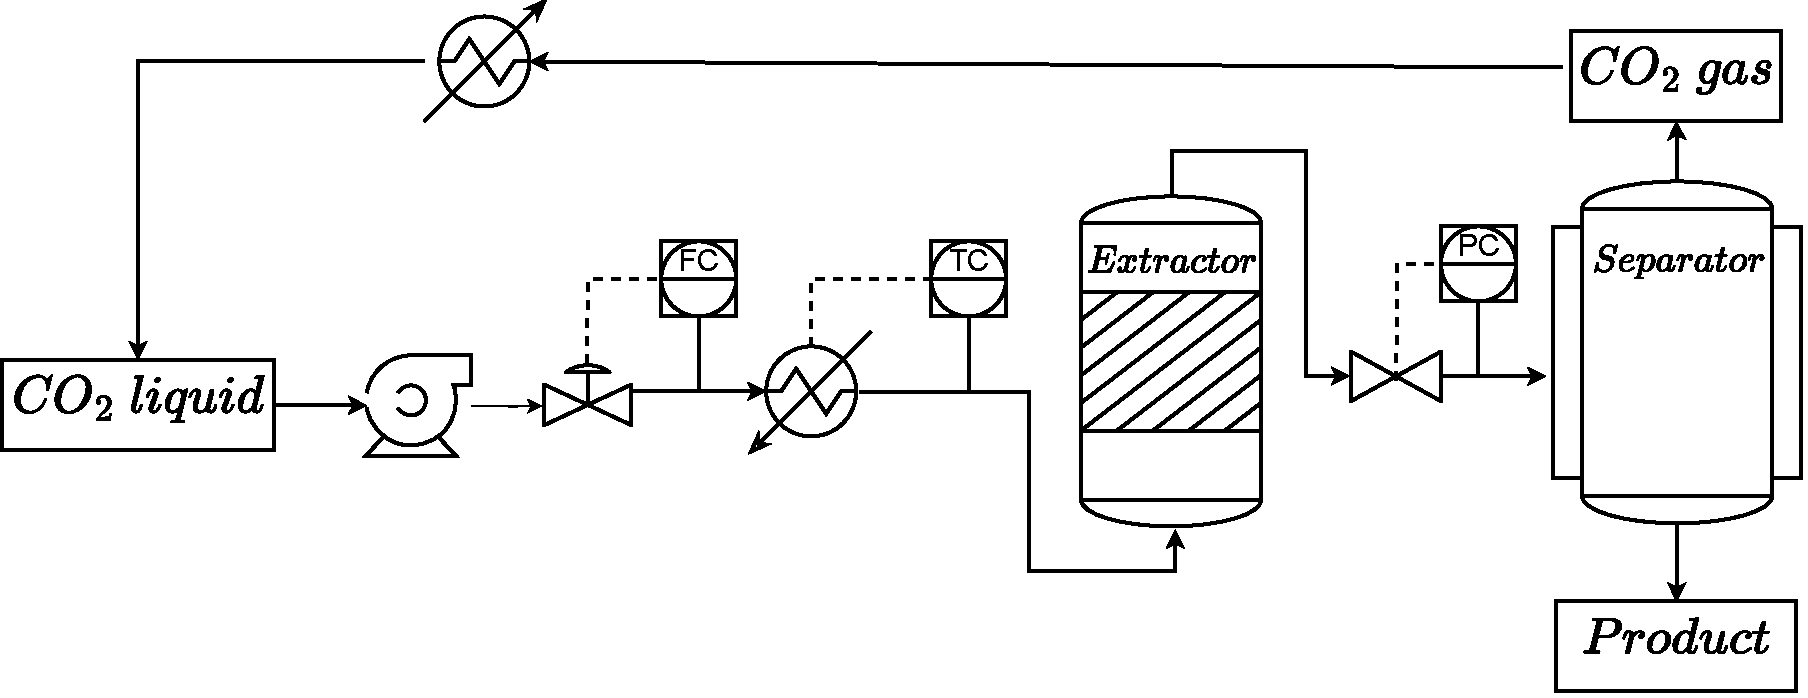
\includegraphics[width=\columnwidth]{Figures/PFD.drawio.pdf}
		\caption{Process flow diagram}
		\label{fig: SFE_drawing}
	\end{figure}
		
	This study focuses on finding a process model for the extraction of natural substances from solid materials using supercritical fluids, with a particular emphasis on supercritical CO$_2$. The approach involves estimating the solvent properties through thermodynamic relationships and determining the extraction kinetic parameters via a series of experiments conducted under a variety of conditions. The maximum likelihood estimation is employed to solve the parameter estimation problem. Later, the correlations between parameters and operating conditions are proposed.
		
\end{document}